\chapter{Generic Cryptographic Interface}
As explained in chapter \ref{motiv}, this interface should be implemented
between the application and the cryptographic provider in the project
\embtls for example. The interface has to be optimized for other projects
too.\newline That's why this interface should have a basis of cryptography which can
be easily adaptable for other projects and easily modifiable for other
providers.\newline
Some constraints are added for the interface, which are:
\begin{itemize}
  \item The link between the keys which could come from the application
  and needed in the provider and inversely.
  \item No hidden states should be written in the function of the interface,
  meaning that no default parameters for an algorithm has to be written
  internally of a function.\newline
\end{itemize}
In several books and on the internet (see Bibliography) the most
important part of cryptography are listed below:
\begin{itemize}
  \item Hash, see \ref{intro_hash} for the definition
  \item Signature, see \ref{intro_sign} for the definition
  \item Cipher (symmetric (see \ref{intro_sym_cipher} for the
  definition) and asymmetric (see \ref{intro_asym_cipher} for the definition), 
  \item Diffie-Hellman, see \ref{intro_dh} for the definition
\end{itemize}
\todo[inline]{What is it - why it's use - how to use - advantage - disadvantage}
\newpage
\section{Context}
\label{gci_ctx}
%1- what we need
% 2- Explain the solution of the context
As explained above, no hidden states should be written in the function of the
interface, meaning that no default parameters for an algorithm has to be written
internally of a function.\newline
For this constraint the principle of context is used.\newline
Through the context, a configuration of an algorithm could be done, meaning that
in the application part, different parameters for this
algorithm can be chosen and this configuration is saved internally in the
interface (see figure \ref{fig:motiv_gci}).\newline
An ID of where is the configuration saved is returned to the application.\newline
When an update has to be done, the ID is given and the interface knows that the
update has to be done with this configuration.\newline
The cryptographic algorithms which the principle of context is used are:
\begin{itemize}
  \item Hash algorithm
  \item Signature algorithm
  \item Cipher algorithm (symmetric and asymmetric)
  \item Diffie-Hellman\newline
\end{itemize}
Through the context, only the parameters added in the configuration are used. No
hidden state is therefore implemented.\newline
The disadvantage of the context is that the user should have good knowledge
of cryptography to configure an algorithm correctly.
The other cryptographic services which don't need a context is because no
configurations are needed to be saved.
\todo[inline]{What is it - why it's use - how to use - advantage - disadvantage}
\newpage
\section{Cryptographic services}
\subsection{Hash}
\label{gci_hash}

The hash algorithm is split into 3 functions in the interface:
\begin{enumerate}
  \item Configuration of the algorithm
  \item Update of a data
  \item Calculation of the digest (finish)
  
\end{enumerate}
\todo[inline]{What is it - why it's use - how to use - advantage - disadvantage}
\subsection*{Configuration}
\begin{figure}[!ht]
\centering
%\frame{
% trim: left, bottom, right, up
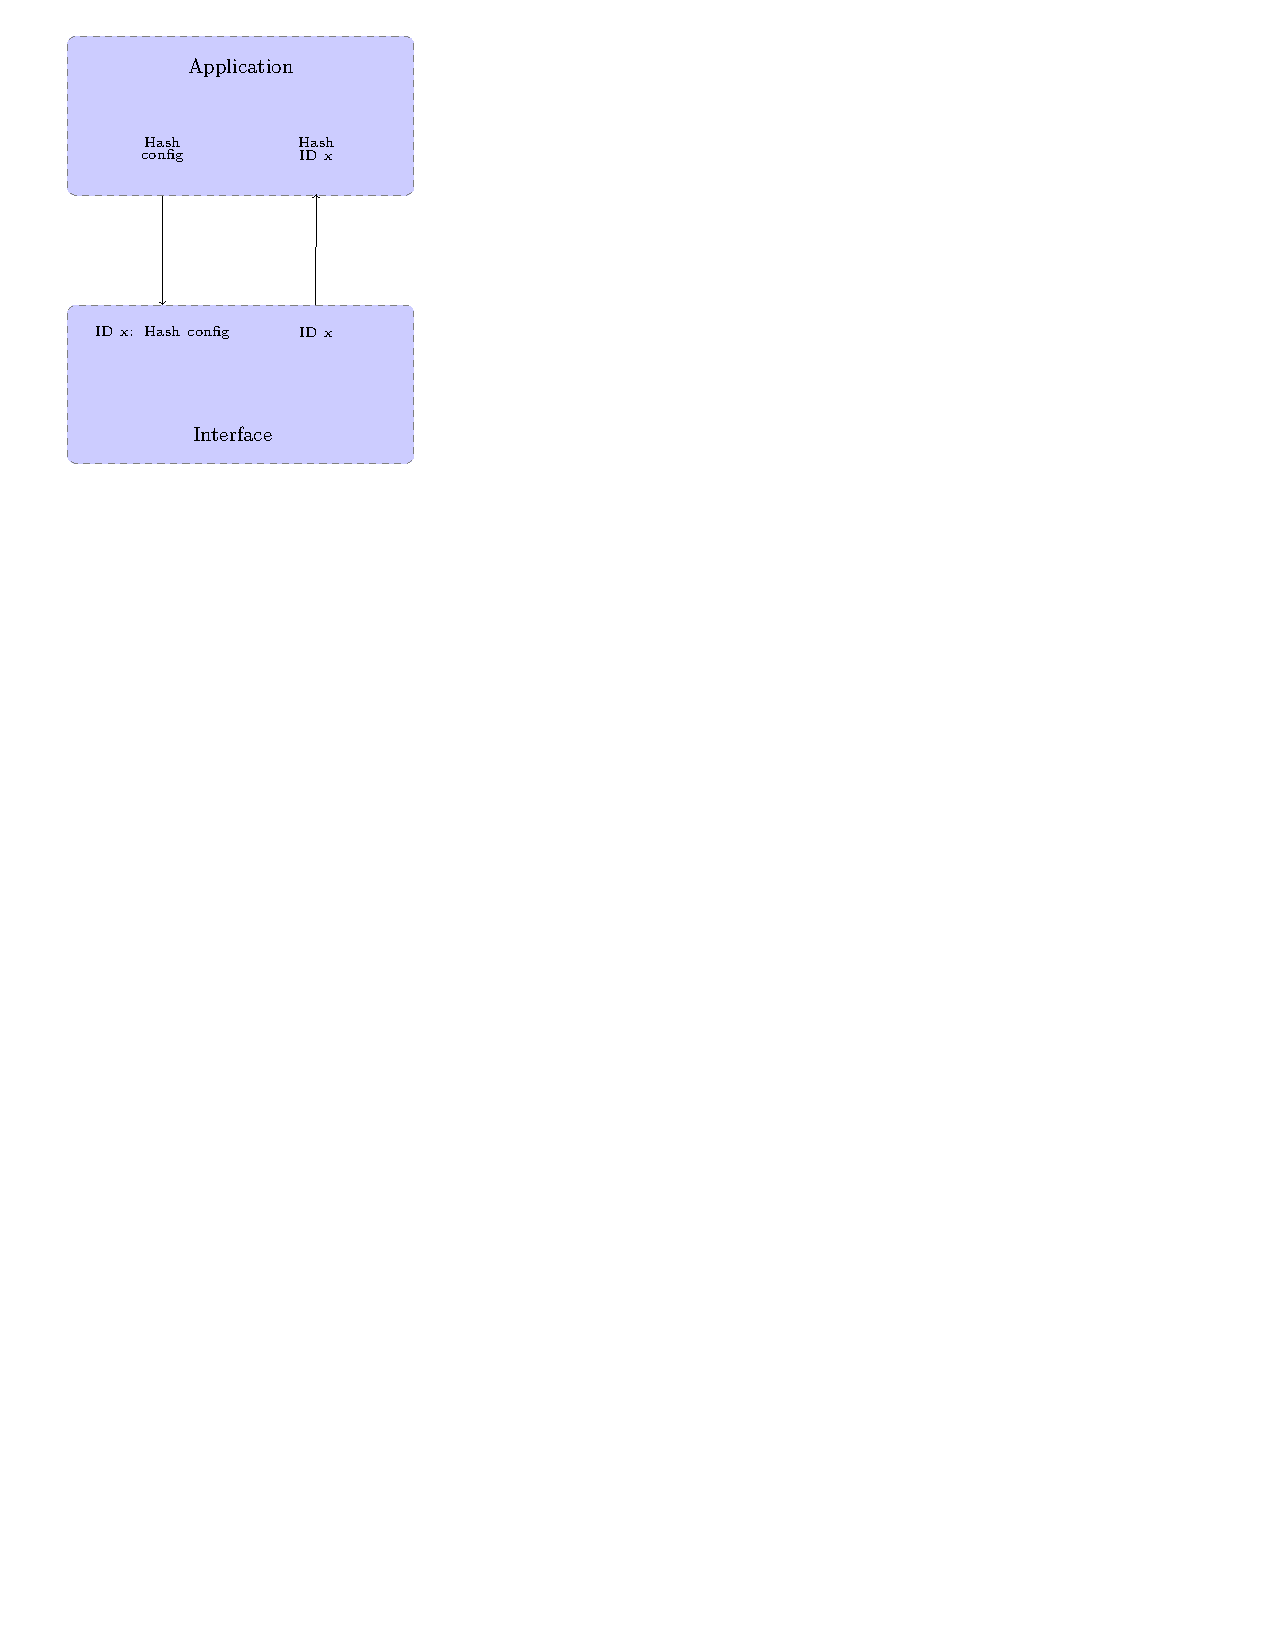
\includegraphics[trim=0cm 20cm 9.5cm 0cm]{figures/hash_example_config.pdf}
\caption{Hash - configuration\newline}
\label{fig:gci_hash_config}
%}
\end{figure}
First part of the hash, it allows to configure the algorithm by only passing
which hash algorithms will be used like:
\begin{itemize}
  \item MD5
  \item SHA1
  \item SHA224
  \item SHA256
  \item SHA384
  \item SHA512
\end{itemize}
As shown on figure \ref{fig:gci_hash_config}, this configuration is than saved
in the interface and an ID of where it's saved is returned to the
application.\newline
\newpage
\subsection*{Update}
\begin{figure}[!ht]
\centering
%\frame{
% trim: left, bottom, right, up
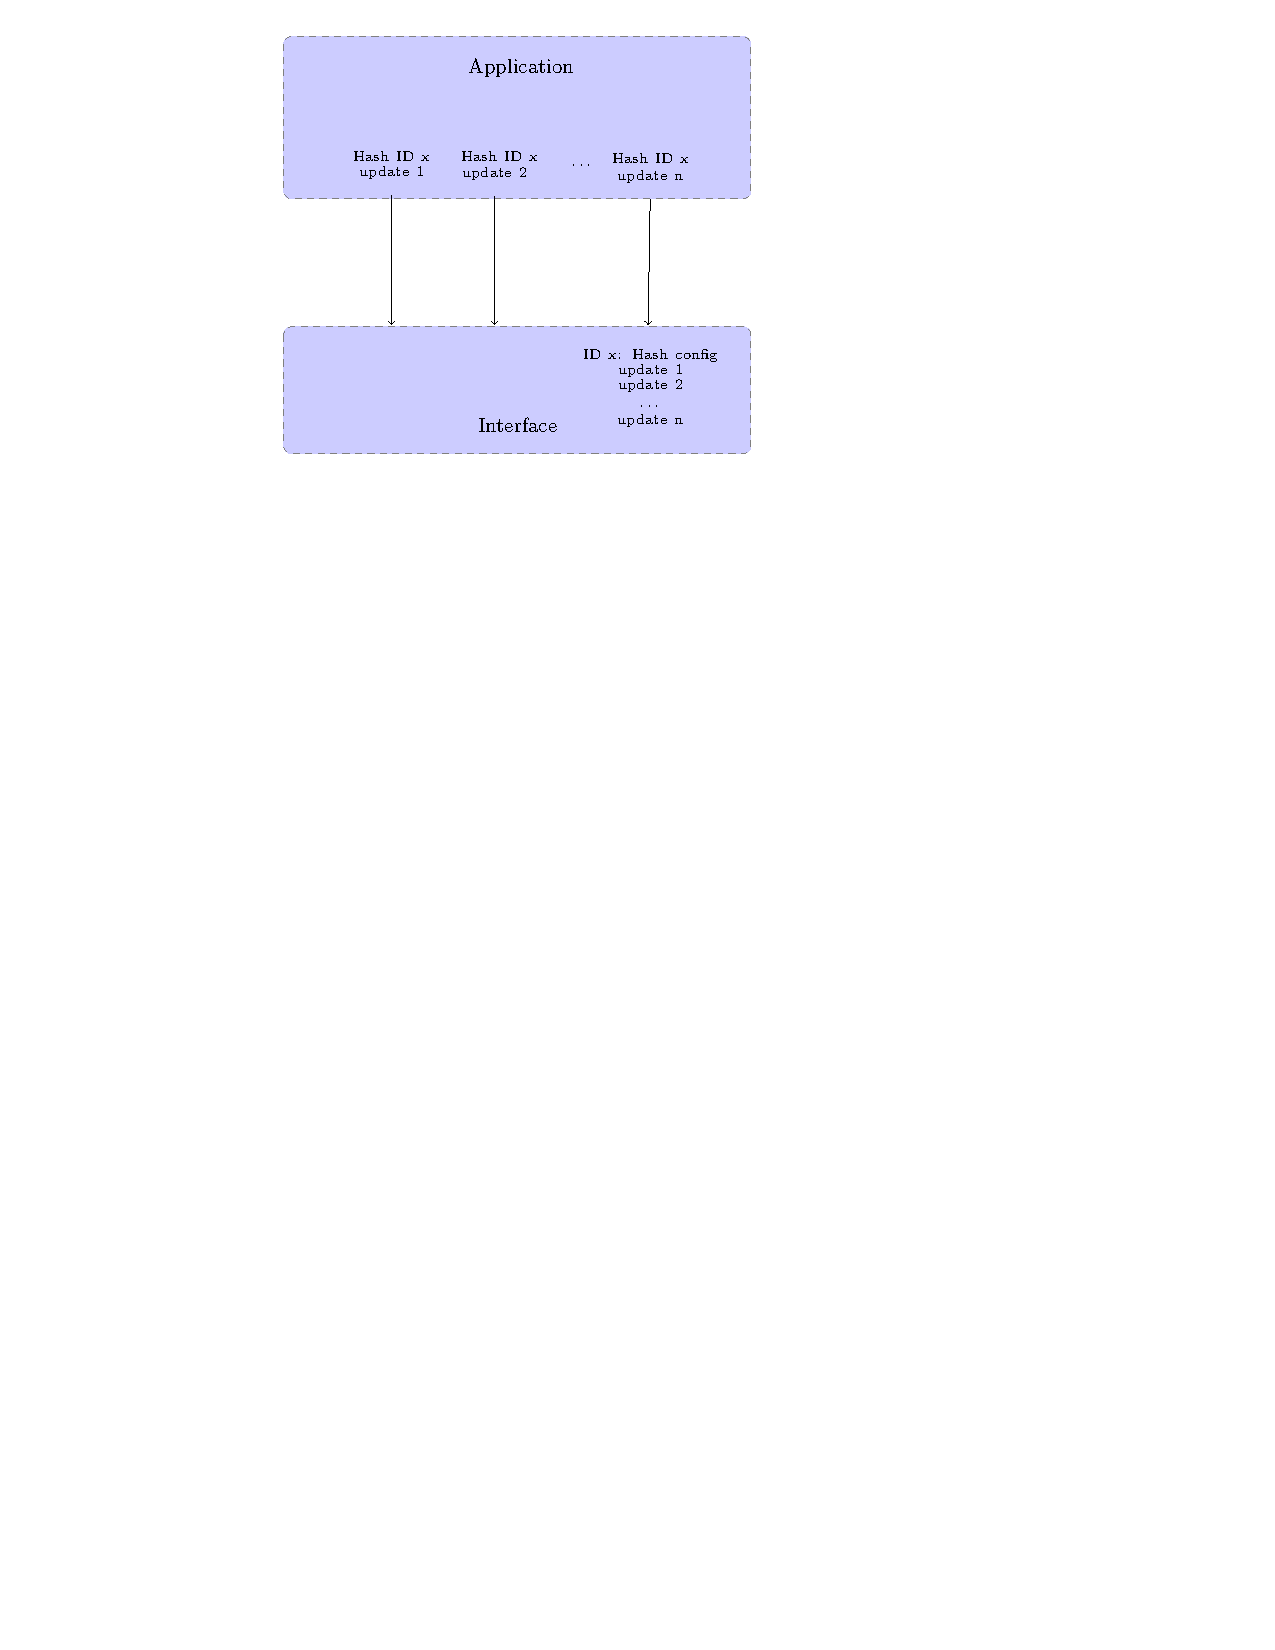
\includegraphics[trim=8cm 20cm 9.5cm 0cm]{figures/hash_example_update.pdf}
\caption{Hash - update\newline}
\label{fig:gci_hash_update}
%}
\end{figure}
When the configuration is done, several updates can be done.\newline
The principle on an update is to add a data which we want to hash.\newline
As shown on figure \ref{fig:gci_hash_update} the ID received in the
configuration part has to be used to add a data.\newline
Through this ID, the interface knows that the data has to be hashed with the
configuration saved at this ID.\newline
\newpage
\subsection*{Finish}
\begin{figure}[!ht]
\centering
%\frame{
% trim: left, bottom, right, up
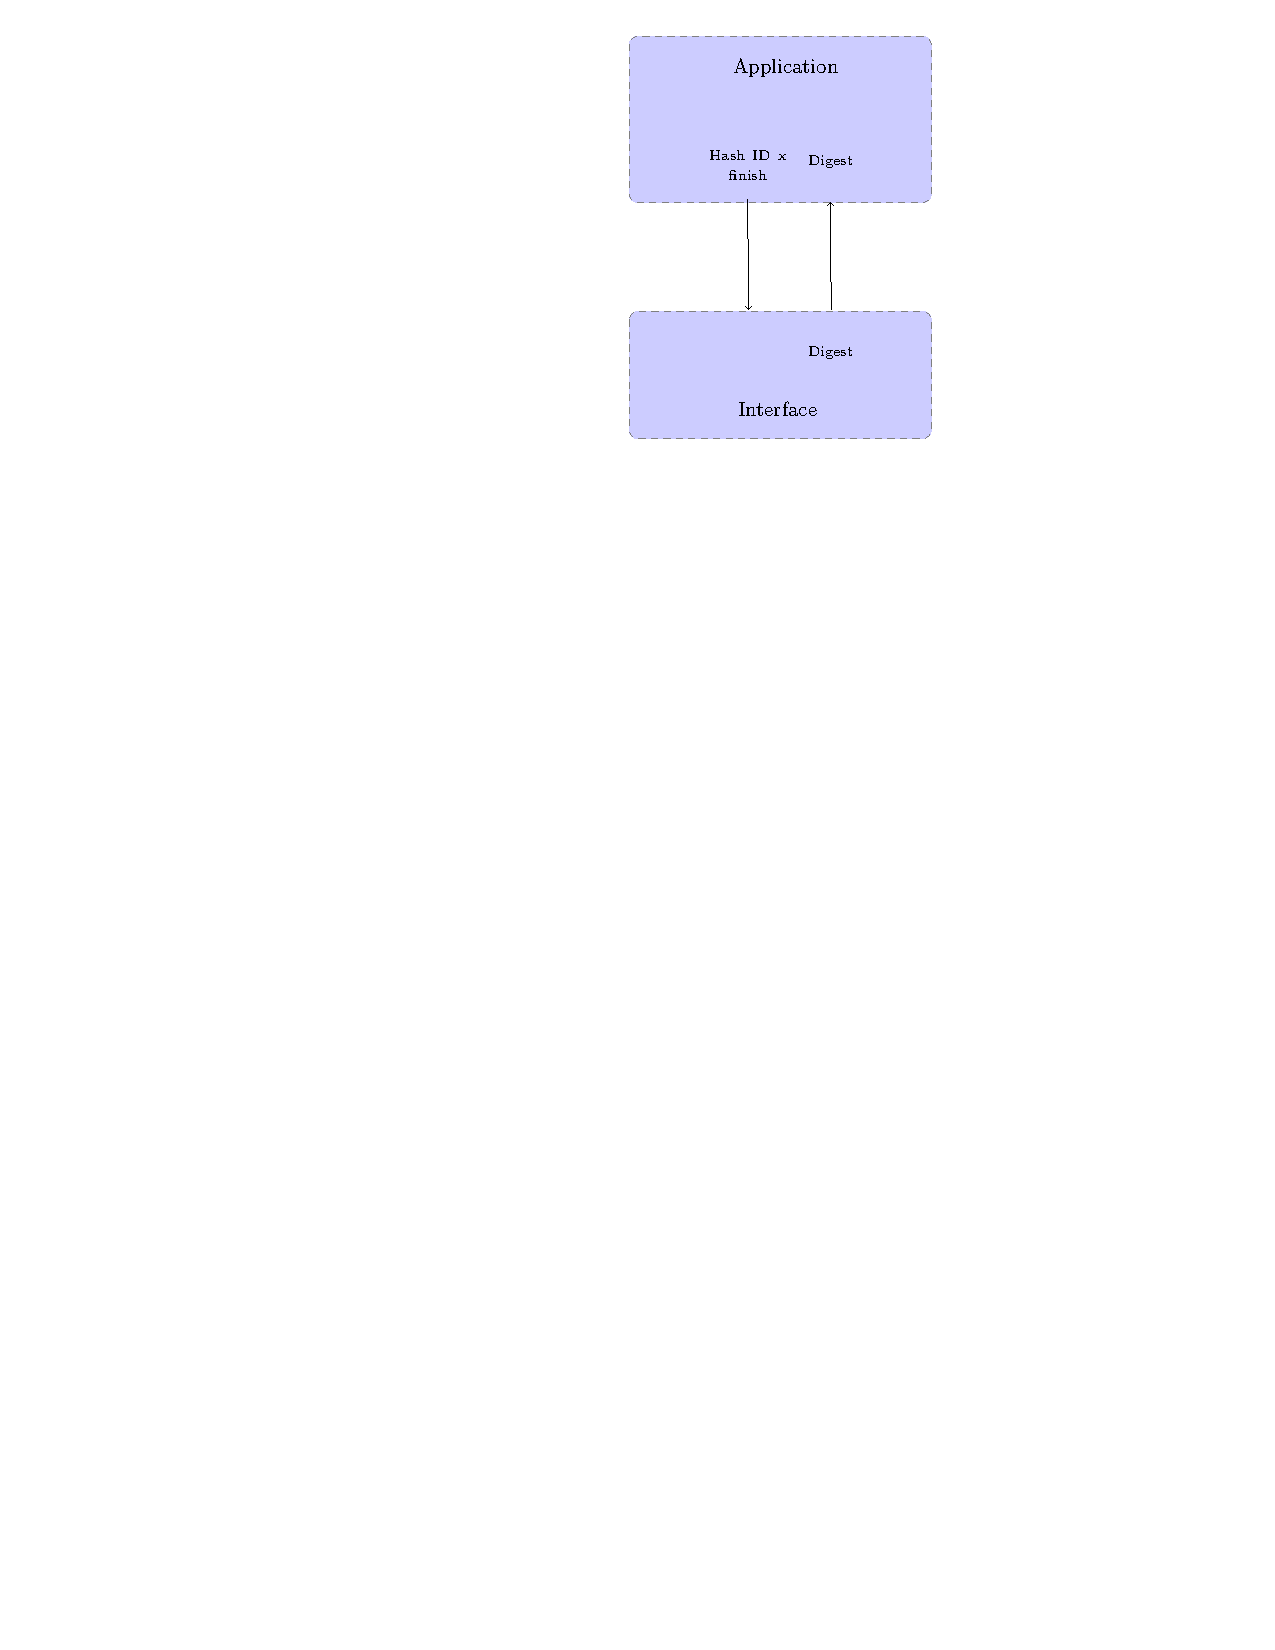
\includegraphics[trim=18.5cm 20cm 9.5cm 0cm]{figures/hash_example_finish.pdf}
\caption{Hash - finish\newline}
\label{fig:gci_hash_finish}
%}
\end{figure}
Last part of the hash is the calculation of the digest\newline
As shown in figure \ref{fig:gci_hash_finish}, by passing the ID which contains
the configuration and all the updated data, the interface will, through the provider, calculate the digest.\newline
One of the disadvantages of this part is when the digest is calculated, all the
updated data and the configuration are lost, meaning that we cannot use them
again to calculate another hash with other data.\newline
This problem is solved in chapter \ref{gci_cl_ctx}
\newpage
\subsection{Generate key pair}
\label{gci_gen_key}
To use other parts of cryptography like signatures and cipher, keys
should be generated.\newline
Only key pairs are generated, meaning that only public and private keys and no
symmetric/shared key.\newline
To get a symmetric key see chapter symmetric cipher (\ref{gci_sym_ciph} or
diffie-hellman (\ref{gci_dh}).\newline
The type of key pair could be:
\begin{itemize}
  \item RSA key pair
  \item DSA key pair
  \item ECDSA key pair (Elliptic curve)
\end{itemize}
For the configuration of a key pair the type of key pair has to be chosen with
one listed above.\newline
Each one has different configurations:
\begin{itemize}
  \item For a RSA key pair, the size of the key should be configured
  \item For a DSA key pair, the domain parameters should be configured (see the
  documentation of the interface in the Appendix for more details)
  \item For ECDSA key pair, the type of elliptic curve has to be given
\end{itemize}
The keys are returned with an ID. For more details on how to get the keys see
the key management \ref{gci_key_mng}
\todo[inline]{What is it - why it's use - how to use - advantage - disadvantage}.
\newpage
\subsection{Signature}
\label{gci_sign}
As some specifications of certain provider, the signature has two possibilities
of use:
\begin{enumerate}
  \item generate a signature
  \item verification of a signature\newline
\end{enumerate}
Each one is split into three functions:
\begin{itemize}
  \item Configuration of the signature
  \item Update data
  \item Generate a signature/Verify a signature\newline
\end{itemize}
Through this algorithm the Message Authentication Code (MAC) can be used
too.
\todo[inline]{What is it - why it's use - how to use - advantage - disadvantage}
\newpage
\subsection*{Configuration}
\begin{figure}[!ht]
\centering
%\frame{
% trim: left, bottom, right, up
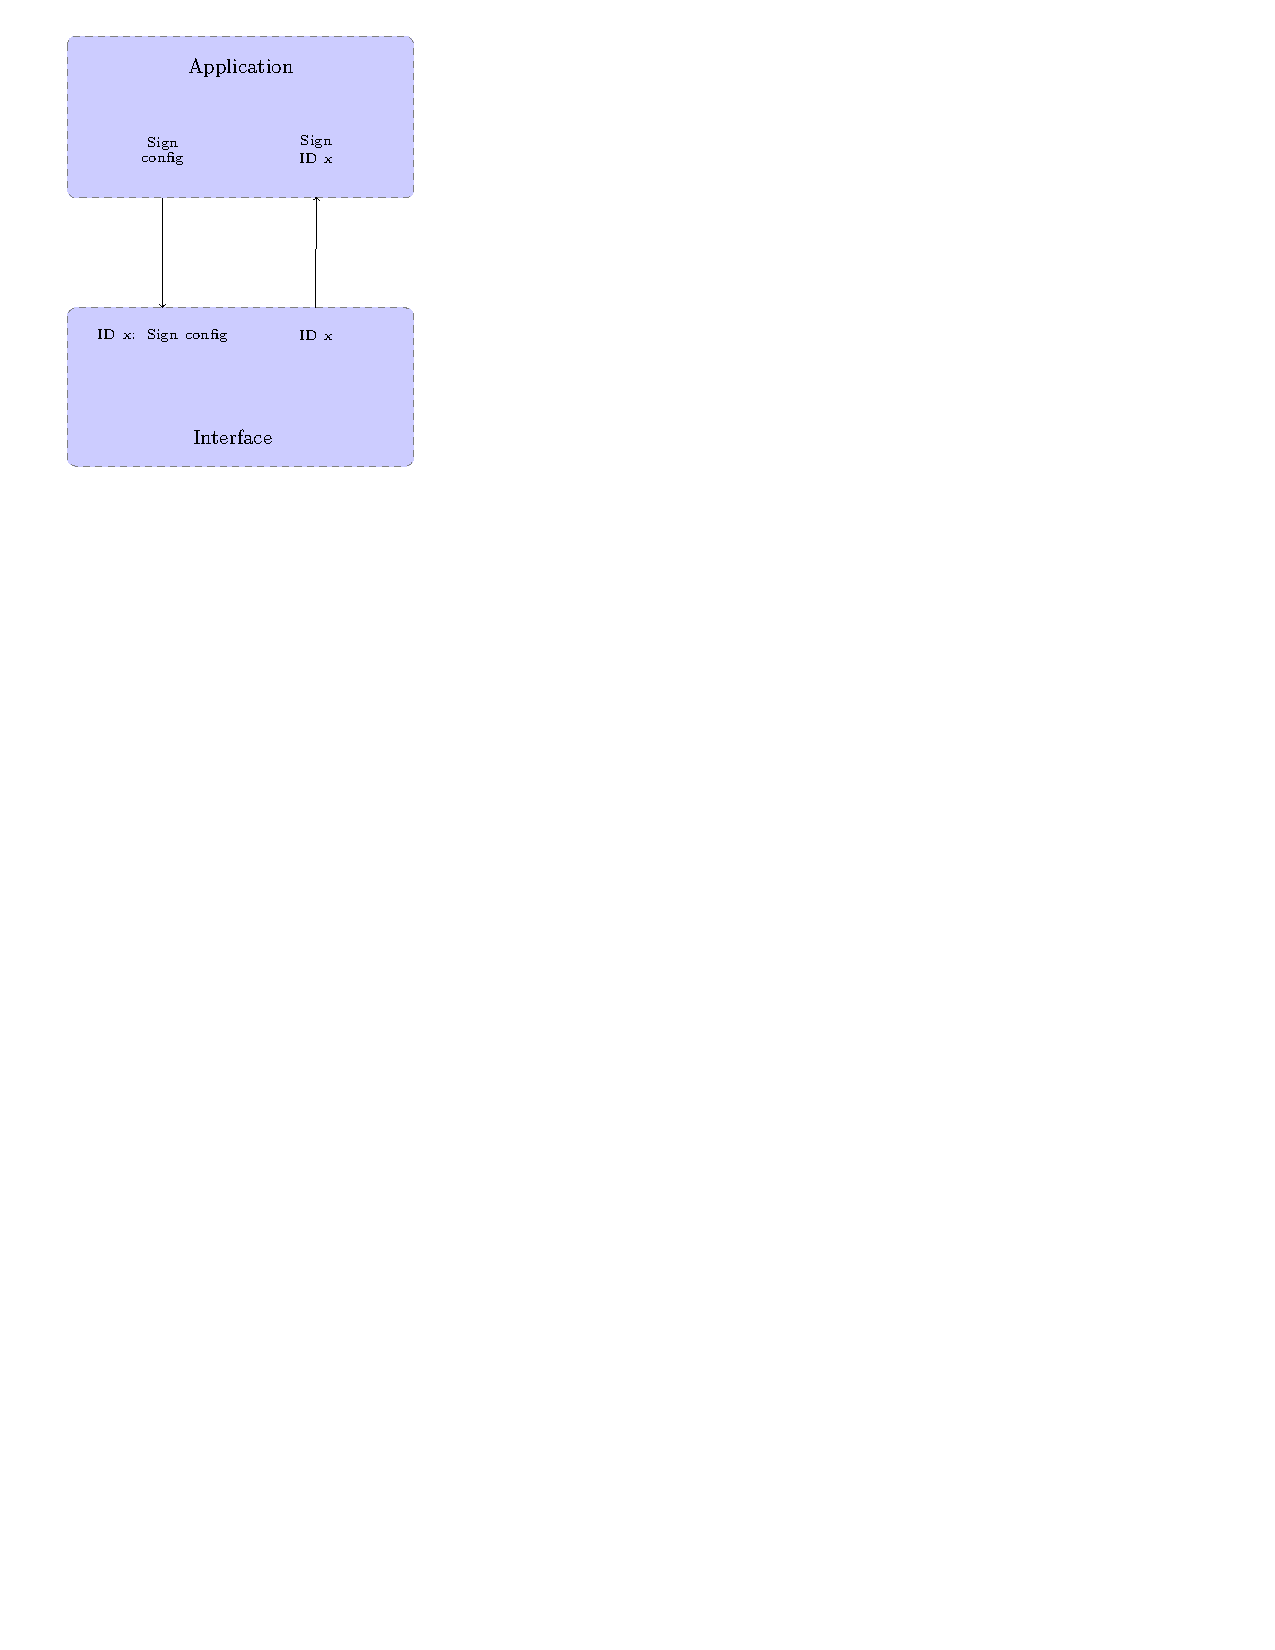
\includegraphics[trim=0cm 20cm 9.5cm 0cm]{figures/sign_example_config.pdf}
\caption{Signature - configuration\newline}
\label{fig:gci_sign_config}
%}
\end{figure}
For the generation and verification of a signature this part is the same (only
the name of the function changes).\newline
First should the signature be configured.\newline
Several parameters has to be configured which are:
\begin{itemize}
  \item the signature/MAC algorithm, which could be:
  \begin{itemize}
    \item RSA
    \item DSA
    \item ECDSA
    \item MAC
    \item CMAC
    \item HMAC
  \end{itemize}
  \item A hash algorithm, if in the updated data should be first hashed before
  signing, or if the HMAC algorithm is used
  \item The padding, if the RSA algorithm is used
  \item The block mode, the padding and the initialization vector, if the CMAC
  algorithm is used
  \item The private key, if RSA, DSA or ECDSA is used to generate a signature or
  the public key if the same algorithm is used to verify a signature
\end{itemize}
As shown figure \ref{fig:gci_sign_config}, when the configuration is done, this
one is saved in the interface and an ID of where is this configuration saved, is
returned to the application.\newline
\subsection*{Update}
\begin{figure}[!ht]
\centering
%\frame{
% trim: left, bottom, right, up
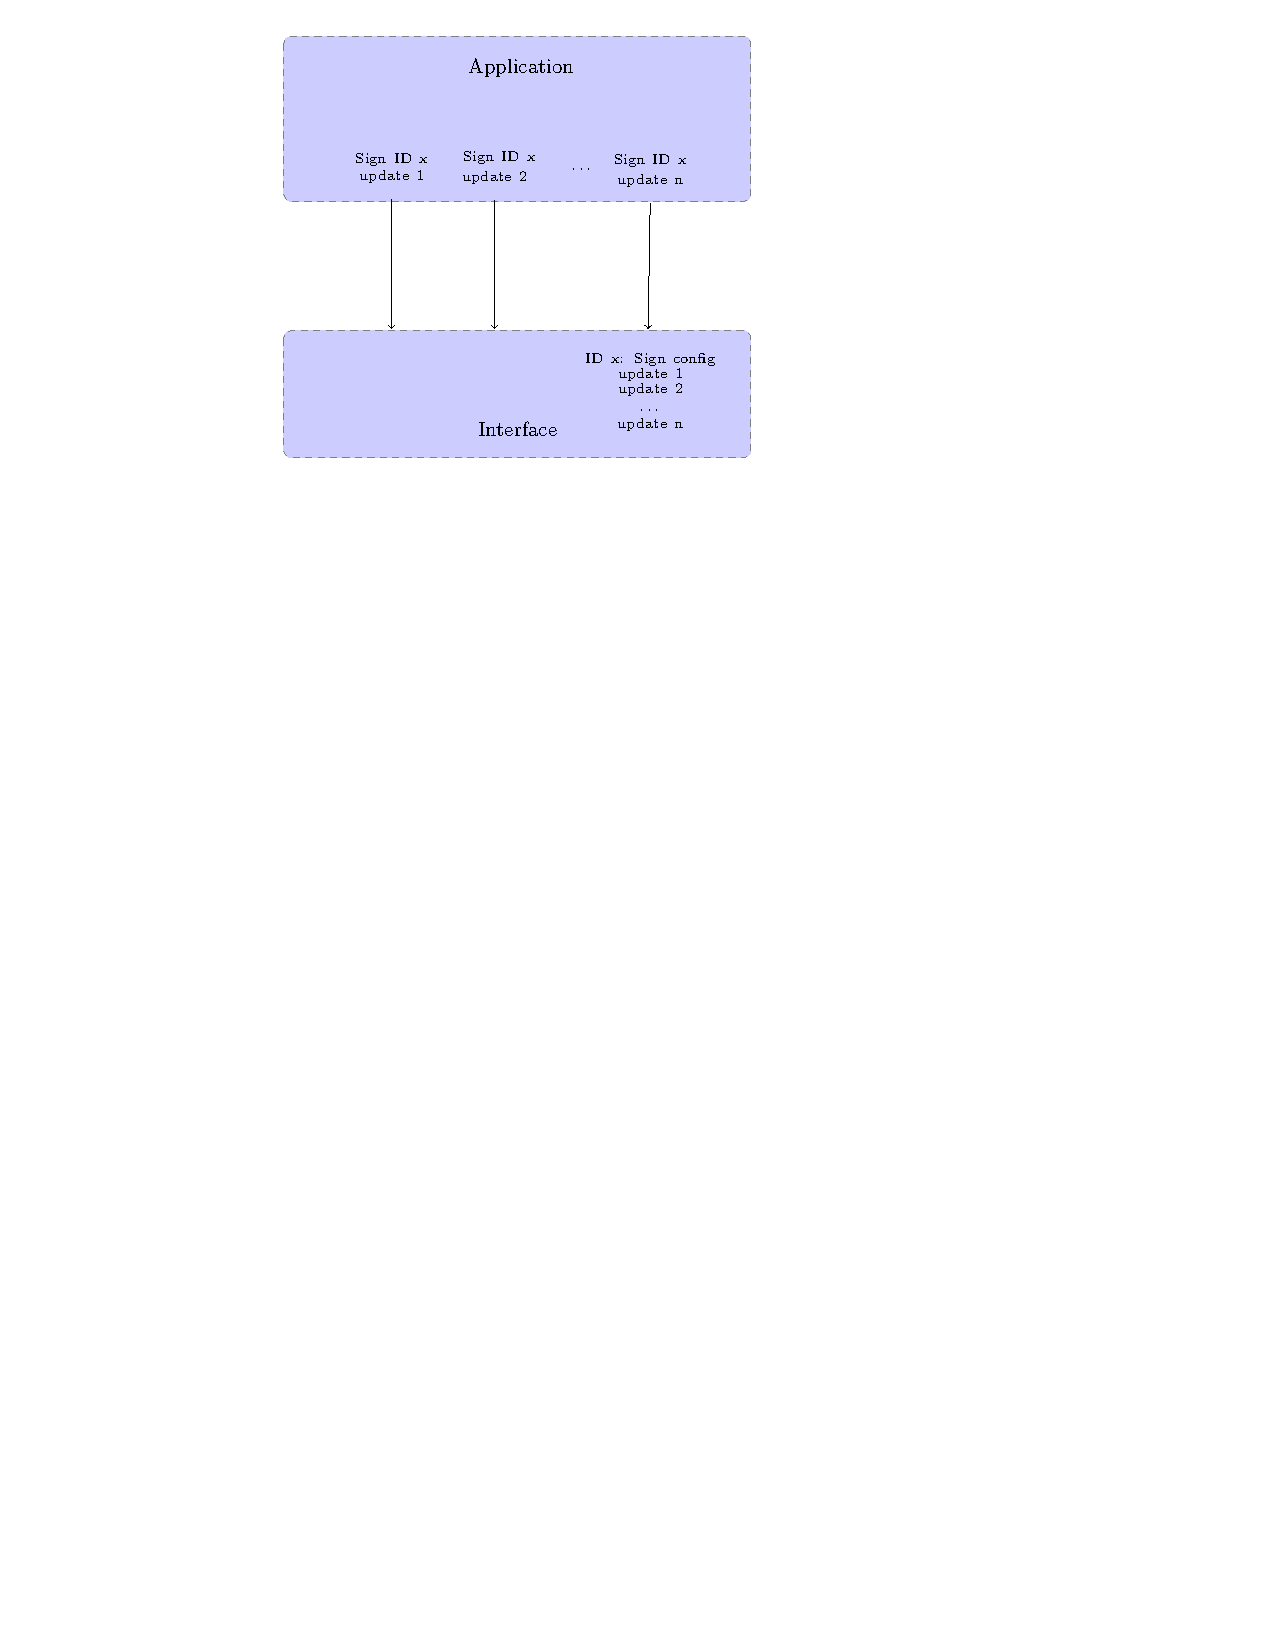
\includegraphics[trim=8cm 20cm 9.5cm 0cm]{figures/sign_example_update.pdf}
\caption{Signature - update\newline}
\label{fig:gci_sign_update}
%}
\end{figure}
When the configuration is done, several updates could be done.\newline
The principle of the update is to add data which will be used to generate or
verify a signature.\newline
As shown in figure \ref{fig:gci_sign_update}, to use the correct configuration,
the ID returned when the configuration is saved, should be used.\newline
\newpage
\subsection*{Finish}
\begin{figure}[!ht]
\centering
%\frame{
% trim: left, bottom, right, up
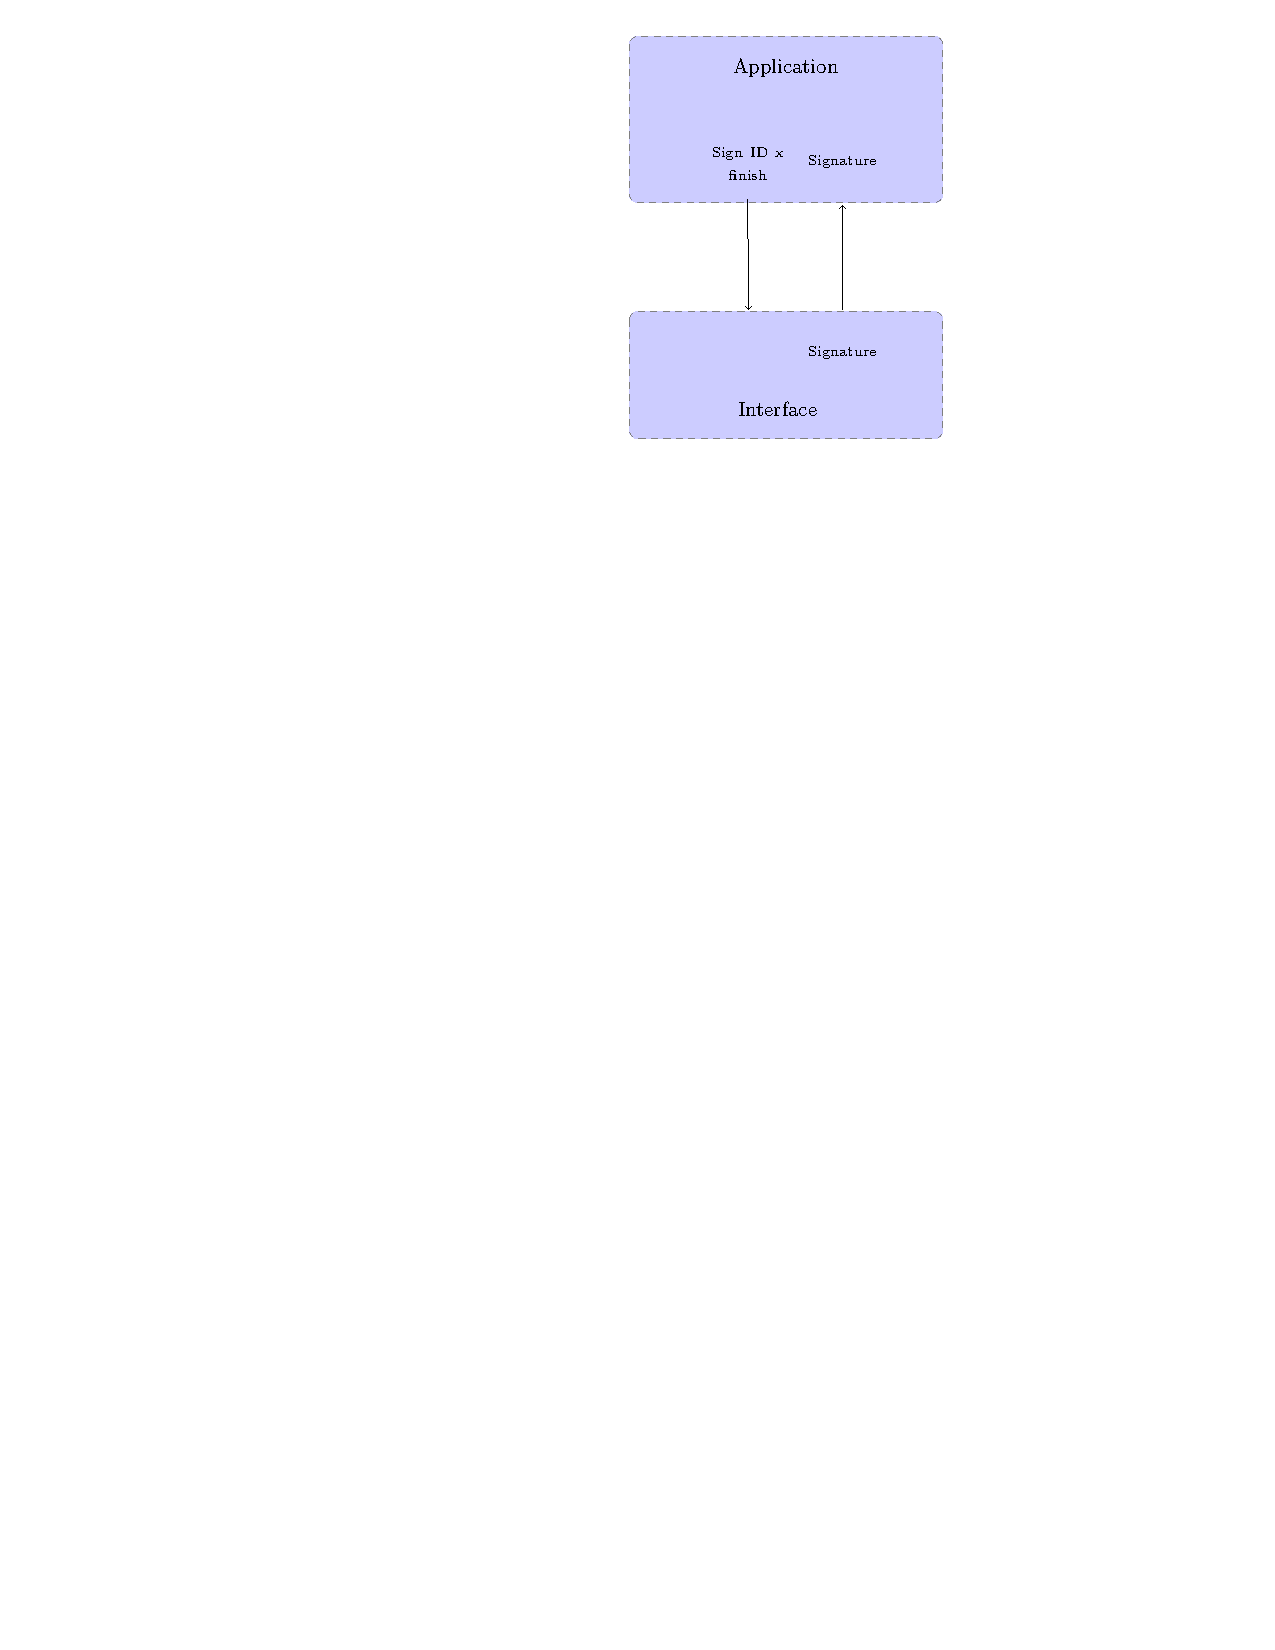
\includegraphics[trim=18.5cm 20cm 9.5cm 0cm]{figures/sign_example_finish.pdf}
\caption{Signature - finish\newline}
\label{fig:gci_sign_finish}
%}
\end{figure}
In this part the generation and the verification are different.\newline
For the generation , the whole updated data and the configuration will be signed
with the private key added in the configuration.\newline
For the verification, the signature we want to verify should be added to the
function.\newline
Than the updated data will be signed, but with the public key.\newline
Than the added signature (which is done with the private key) could be compared
with the ``signature'' computed to verify.\newline
The most important part of the verification is that the private key, which
the signature is done and the public key for the verification, should be
generated together.
\newpage
\subsection{Cipher (symmetric and asymmetric)}
\label{gci_ciph}
A cipher, as explained in \ref{intro_cipher}, which
could be symmetric or asymmetric, is an algorithm for encrypting and decrypting
data.\newline
This concept is therefore used in the interface and split into three main
functions which are:
\begin{itemize}
  \item Configuration of the cipher
  \item Encryption of a plaintext
  \item Decryption of a ciphertext
\end{itemize}
\subsection*{Configuration of the cipher}
Several parameters are to be configured for the cipher algorithm and depends
particularly of which cipher algorithm is used.\newline
The cipher algorithm is split into three main algorithm:
\begin{itemize}
  \item Symmetric stream cipher algorithm\newline
  Today very deprecated but is, however,
implemented in the interface if comparison has to be done.\newline
Only the RC4 stream cipher is implemented in the interface.\newline
Other stream cipher can, however, be easily added in the interface if
needed.\newline
Nothing more as the algorithm has to be configured for the use of
it.\newline
  \item Symmetric block cipher algorithm\newline
  Three kinds of symmetric block cipher algorithms are used today and
therefore implemented in the interface:
\begin{itemize}
  \item Data Encryption Standard (DES)
  \item 3DES, three subsequent DES encryption
  \item Advanced Encryption Standard (AES)  
\end{itemize}
Each symmetric block cipher algorithm needs a mode of operation, named block
mode in the interface, which depends on the size of data we want to
encrypt.\newline
The block mode implemented in the interface are:
\begin{itemize}
  \item Electronic Code Book mode (ECB)
  \item Cipher Block Chaining mode (CBC)
  \item Cipher Feedback mode (CFB)
  \item Output Feedback mode (OFB)
  \item Counter mode (CTR)
  \item Galois Counter Mode (GCM)
\end{itemize}
  \item Asymmetric algorithm\newline
  Only the RSA algorithm is implemented for this part of the interface.\newline
  In practice to use the RSA algorithm this one should use a padding to increase
  the security of it.\newline
  The best known padding in the Public-Key Cryptography Standard (PKCS) and is,
of course, implemented in the interface.\newline  
\end{itemize} 
The most important thing for a cipher is, of course, the key!\newline
For a symmetric cipher, stream or block, the key is only a shared key.\newline
For an asymmetric cipher, if an encryption will be done, a public key should
be added. If a decryption will be done, a private key should be added to the
configuration.
\begin{figure}[!ht]
\centering
%\frame{
% trim: left, bottom, right, up
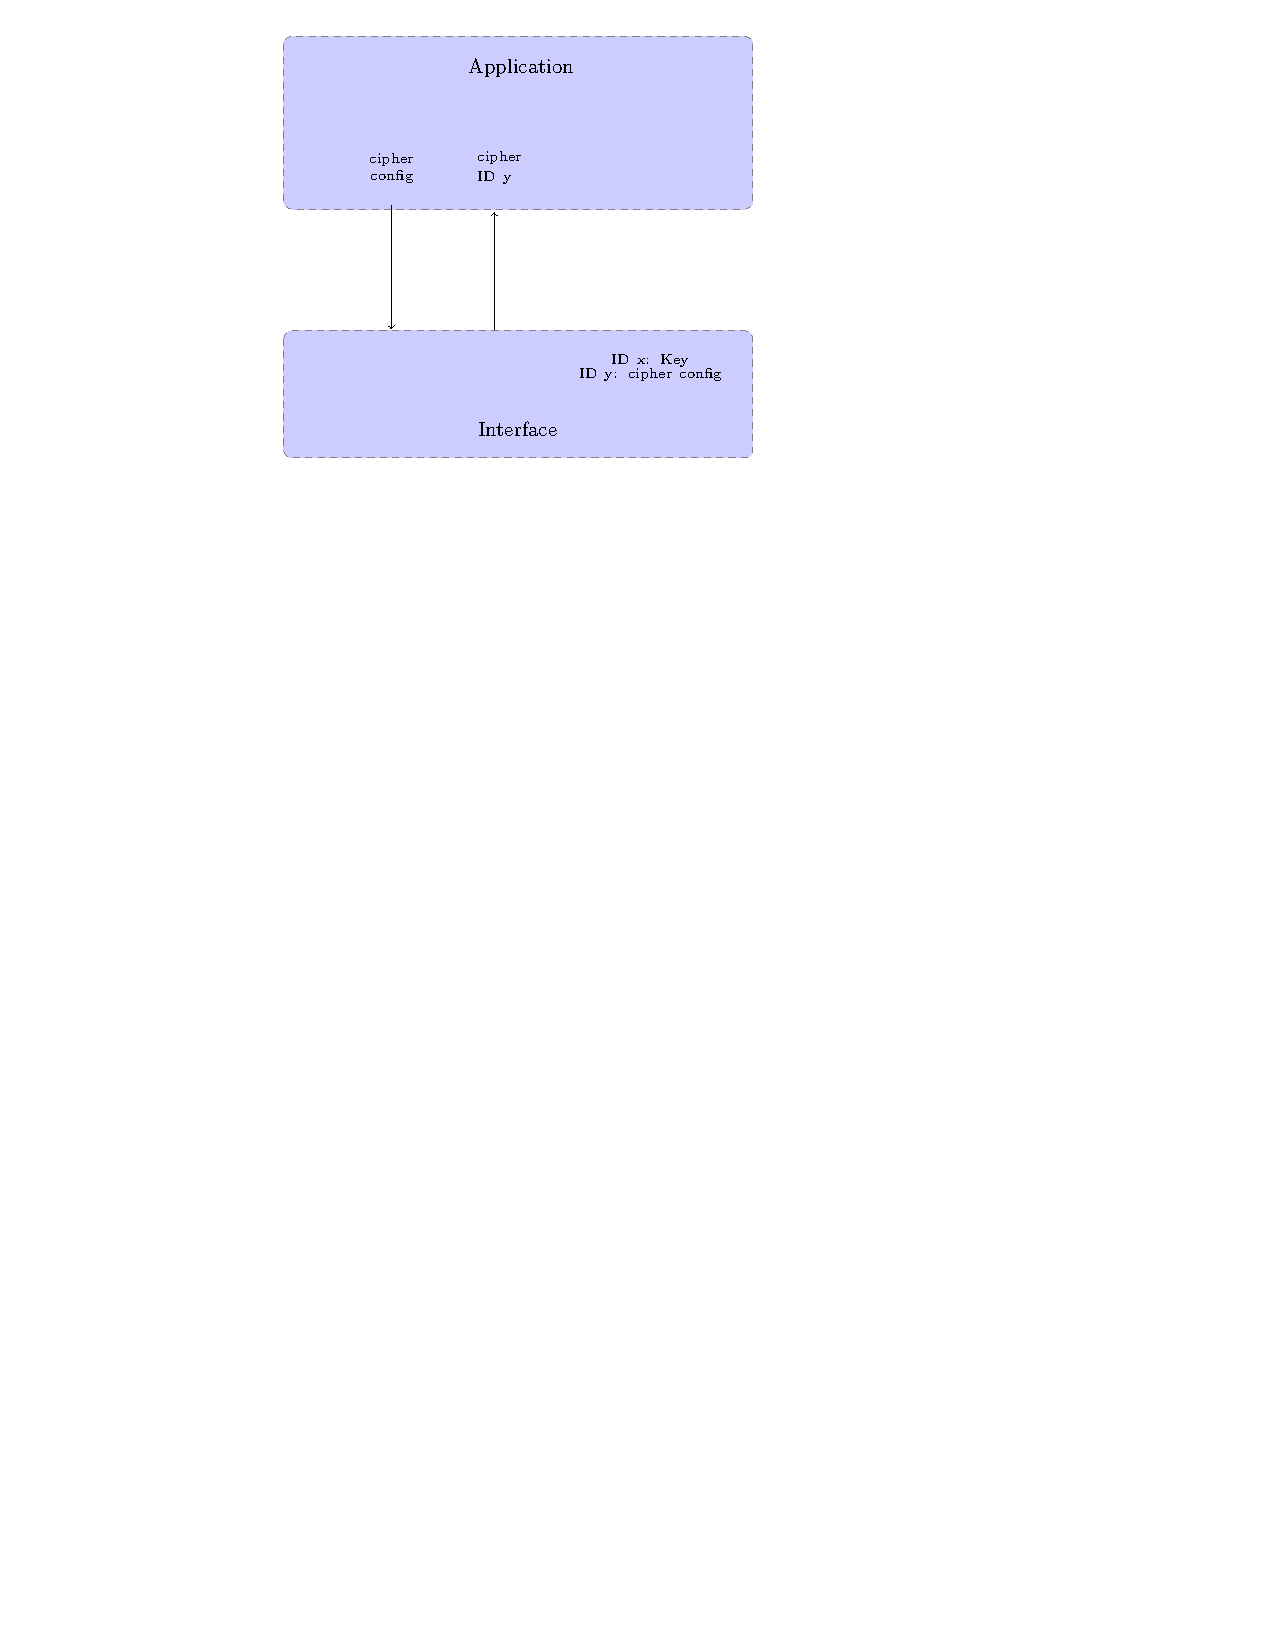
\includegraphics[trim=8.5cm 20cm 9.5cm 0cm]{figures/cipher_example_config.pdf}
\caption{Cipher - configuration\newline}
\label{fig:gci_cipher_config}
%}
\end{figure}
Thenceforth the configuration is done this one should be sent to the interface
which will save it in a context.\newline
The interface returned an ID of the context, which corresponds of where is saved
the configuration, if this one should be used in the future.\newline
The key added to the function is an ID of the key which is already saved in
the interface.\newline
This principle is shown in figure \ref{fig:gci_cipher_config}

\newpage
\subsection*{Encryption of a plaintext}
\begin{figure}[!ht]
\centering
%\frame{
% trim: left, bottom, right, up
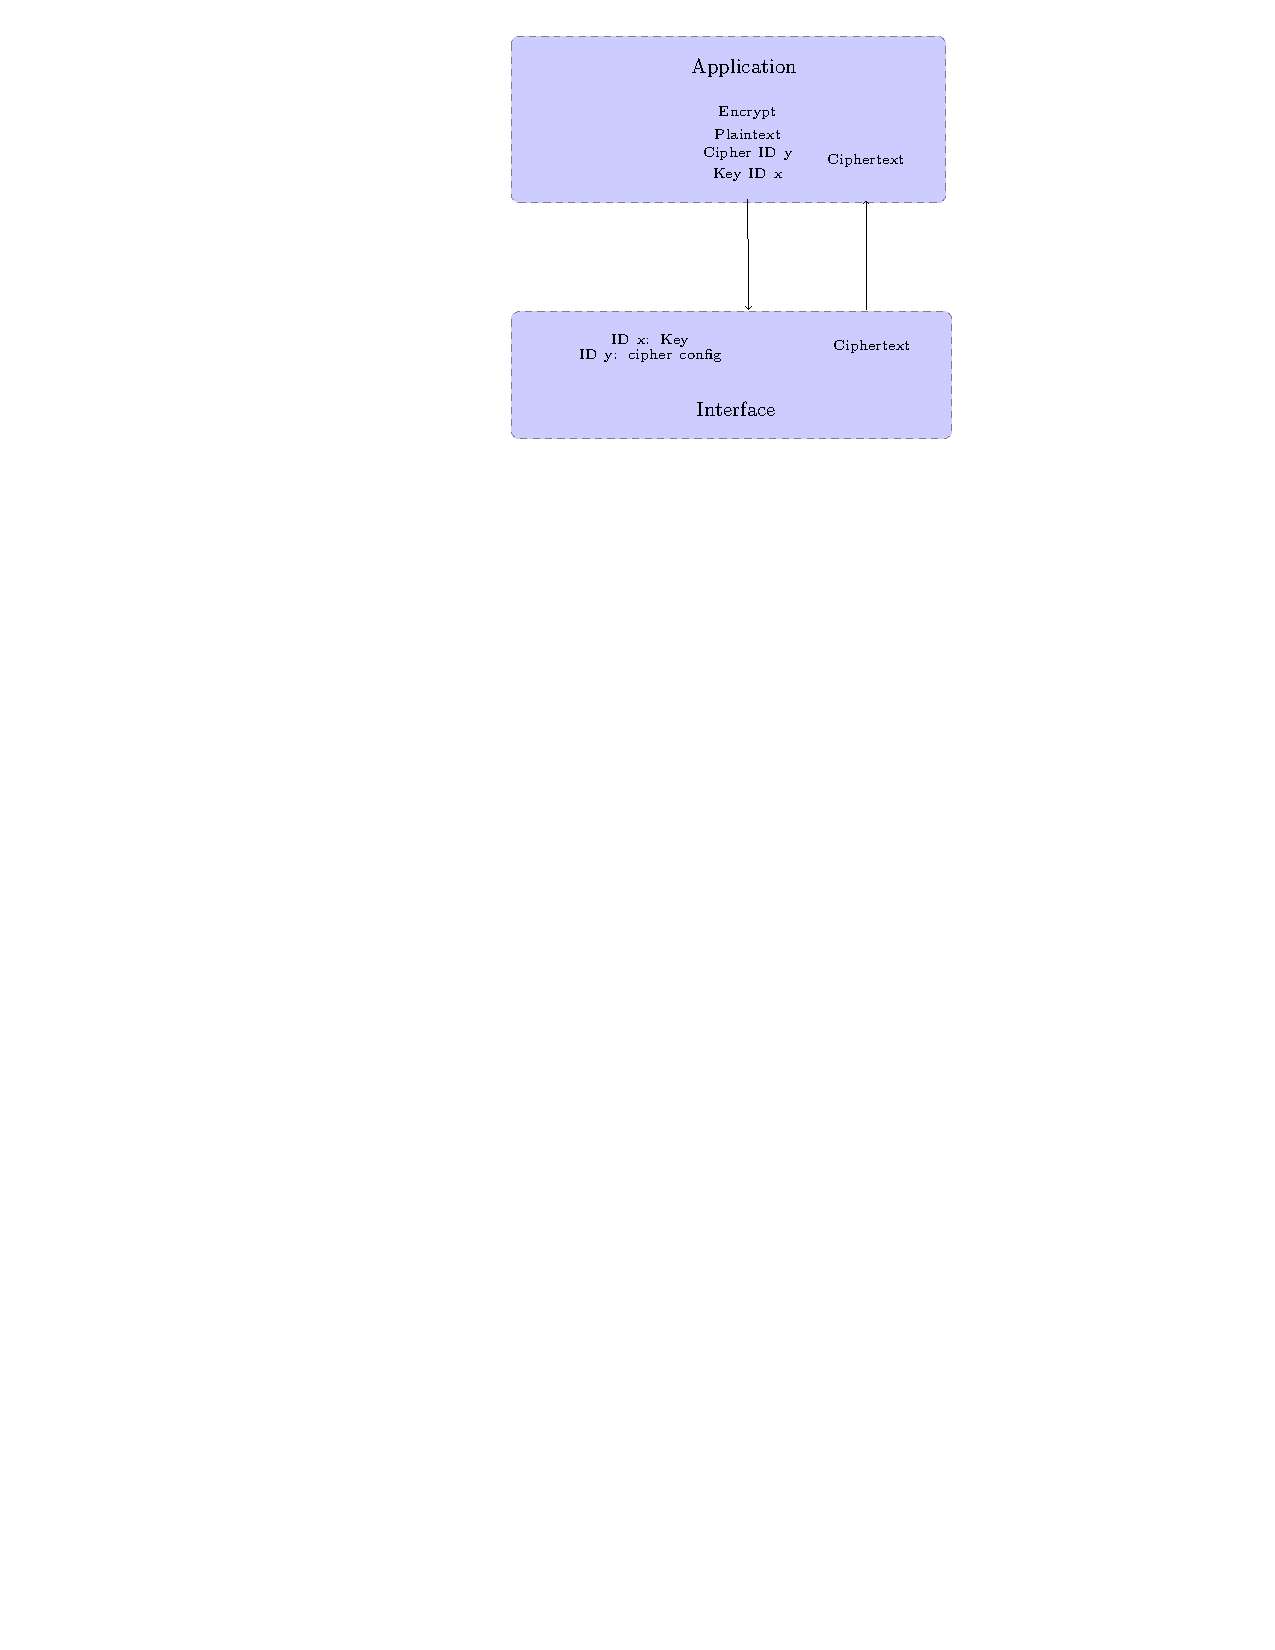
\includegraphics[trim=16cm 20cm 9.5cm 0cm]{figures/cipher_encrypt.pdf}
\caption{Cipher - Encryption\newline}
\label{fig:gci_cipher_encrypt}
%}
\end{figure}
Thenceforth the configuration is done, a encryption can be done.\newline
To encrypt data, the ID of the context (where is the configuration saved)
should be added to the function with the data to encrypt (plaintext).\newline
The interface will, through a provider, calculate the ciphertext of the
plaintext with the configuration saved previously in the context.\newline
This principle is shown figure \ref{fig:gci_cipher_encrypt}
\newpage

\subsection*{Decryption of a ciphertext}
\begin{figure}[!ht]
\centering
%\frame{
% trim: left, bottom, right, up
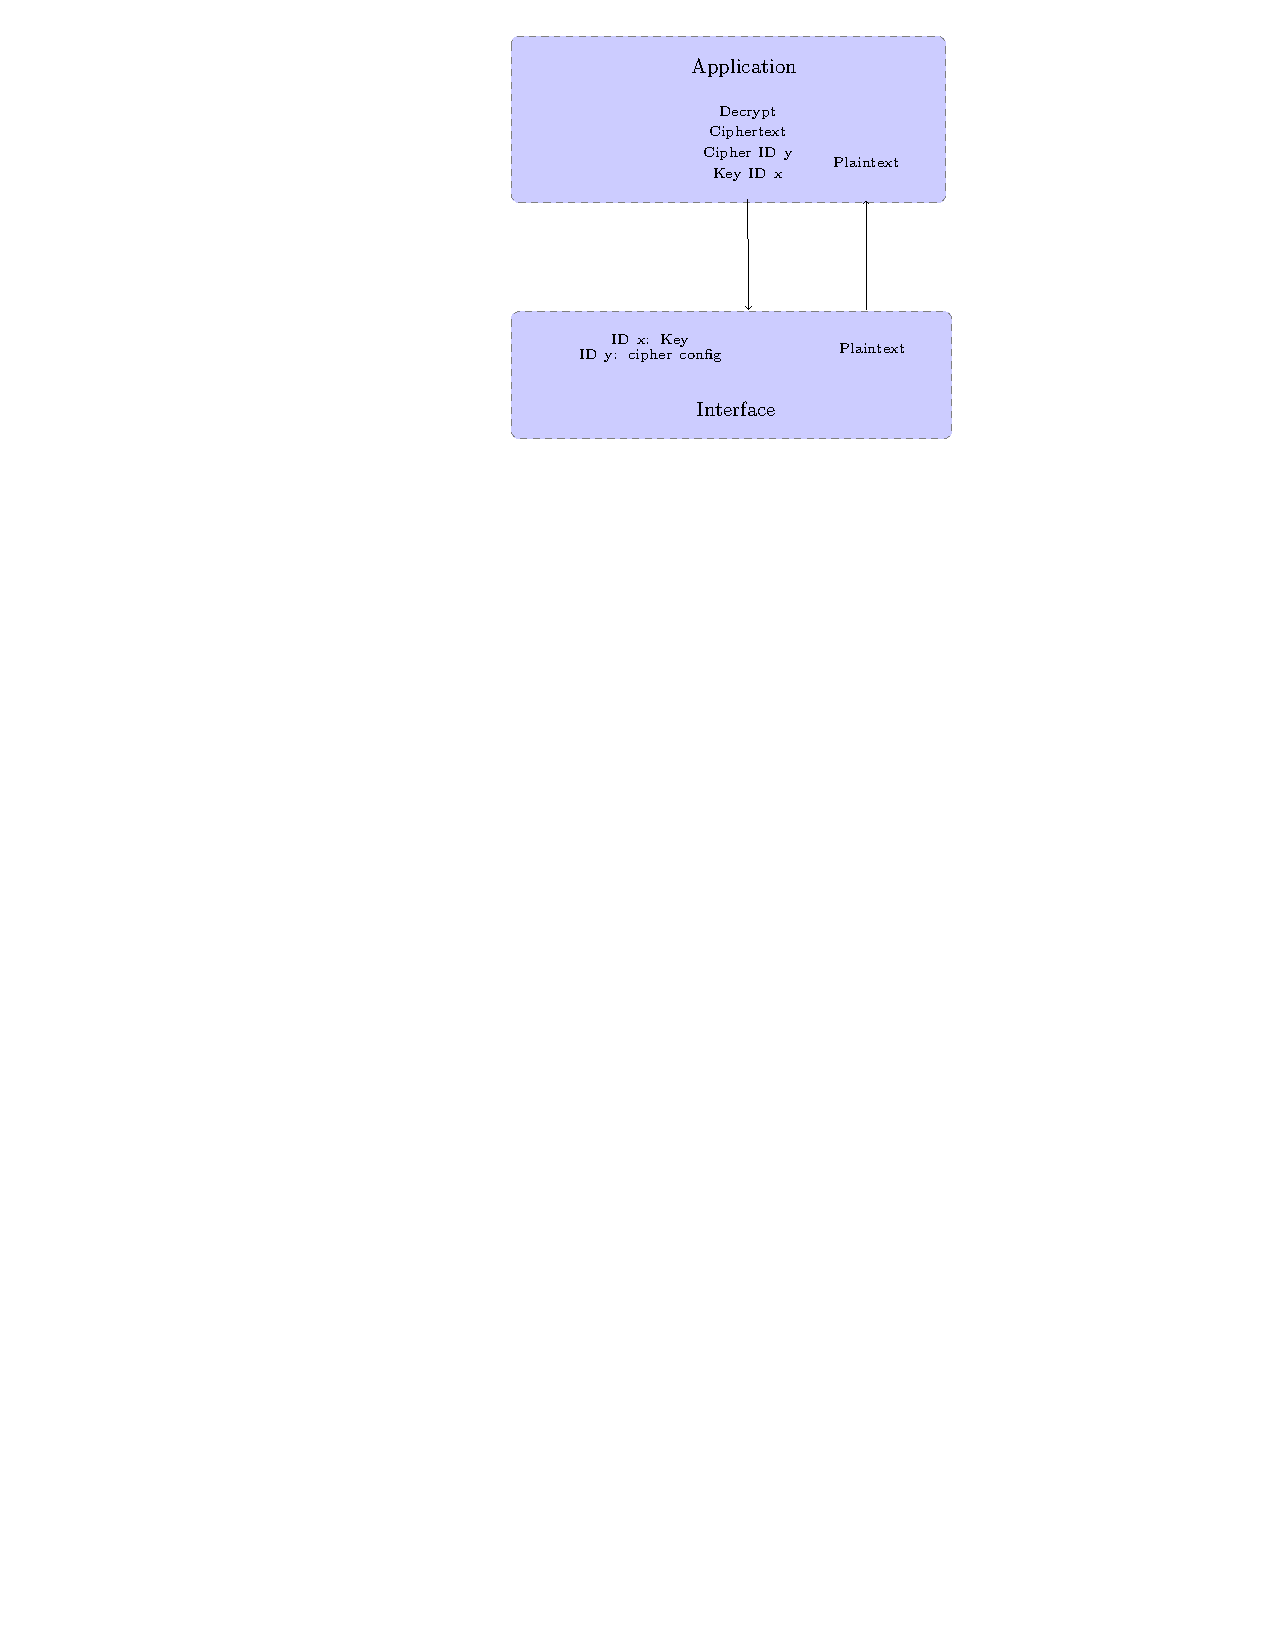
\includegraphics[trim=16cm 20cm 9.5cm 0cm]{figures/cipher_decrypt.pdf}
\caption{Cipher - Decryption\newline}
\label{fig:gci_cipher_decrypt}
%}
\end{figure}
Thenceforth the configuration is done, a decryption can be done.\newline
To decrypt a data, the ID of the context (where is the configuration saved)
should be added to the function with the data to decrypt (ciphertext).\newline
The interface will, through a provider, calculate the plaintext of the
ciphertext with the configuration saved previously in the context.\newline
This principle is shown figure \ref{fig:gci_cipher_decrypt}
\newpage
\subsection{Diffie-Hellman}
\label{gci_dh}
\todo[inline]{What is it - why it's use - how to use - advantage - disadvantage}
\newpage
\subsection{Random number generator}
\label{gci_rng}
\todo[inline]{What is it - why it's use - how to use - advantage - disadvantage}
\newpage
\section{Clone of context}
\label{gci_cl_ctx}
As explained in \ref{gci_hash} and \ref{gci_sign} when the digest (for the hash)
and the signature (for the signature) is calculated, no more data can be added
to the context.\newline
This is a problem for the use of this interface in TLS projects (\embtls for
example).\newline
Several solutions was introduced which are:
\begin{enumerate}
  \item Use two contexts at the same time.\newline
  This wasn't very efficient, because we should know at the beginning the
  number of times a digest will be calculated, which determines the amount of
  context we have to create at the beginning.
  \item Create a context when the digest is calculated.\newline
  The disadvantage of this idea was that the whole data use previously has to be
  saved. For systems, like embedded systems, with memory constraints, this is
  not practicable.
  \item Clone the context. This is the kept solution.\newline
\end{enumerate}
\begin{figure}[!ht]
\centering
%\frame{
% trim: left, bottom, right, up
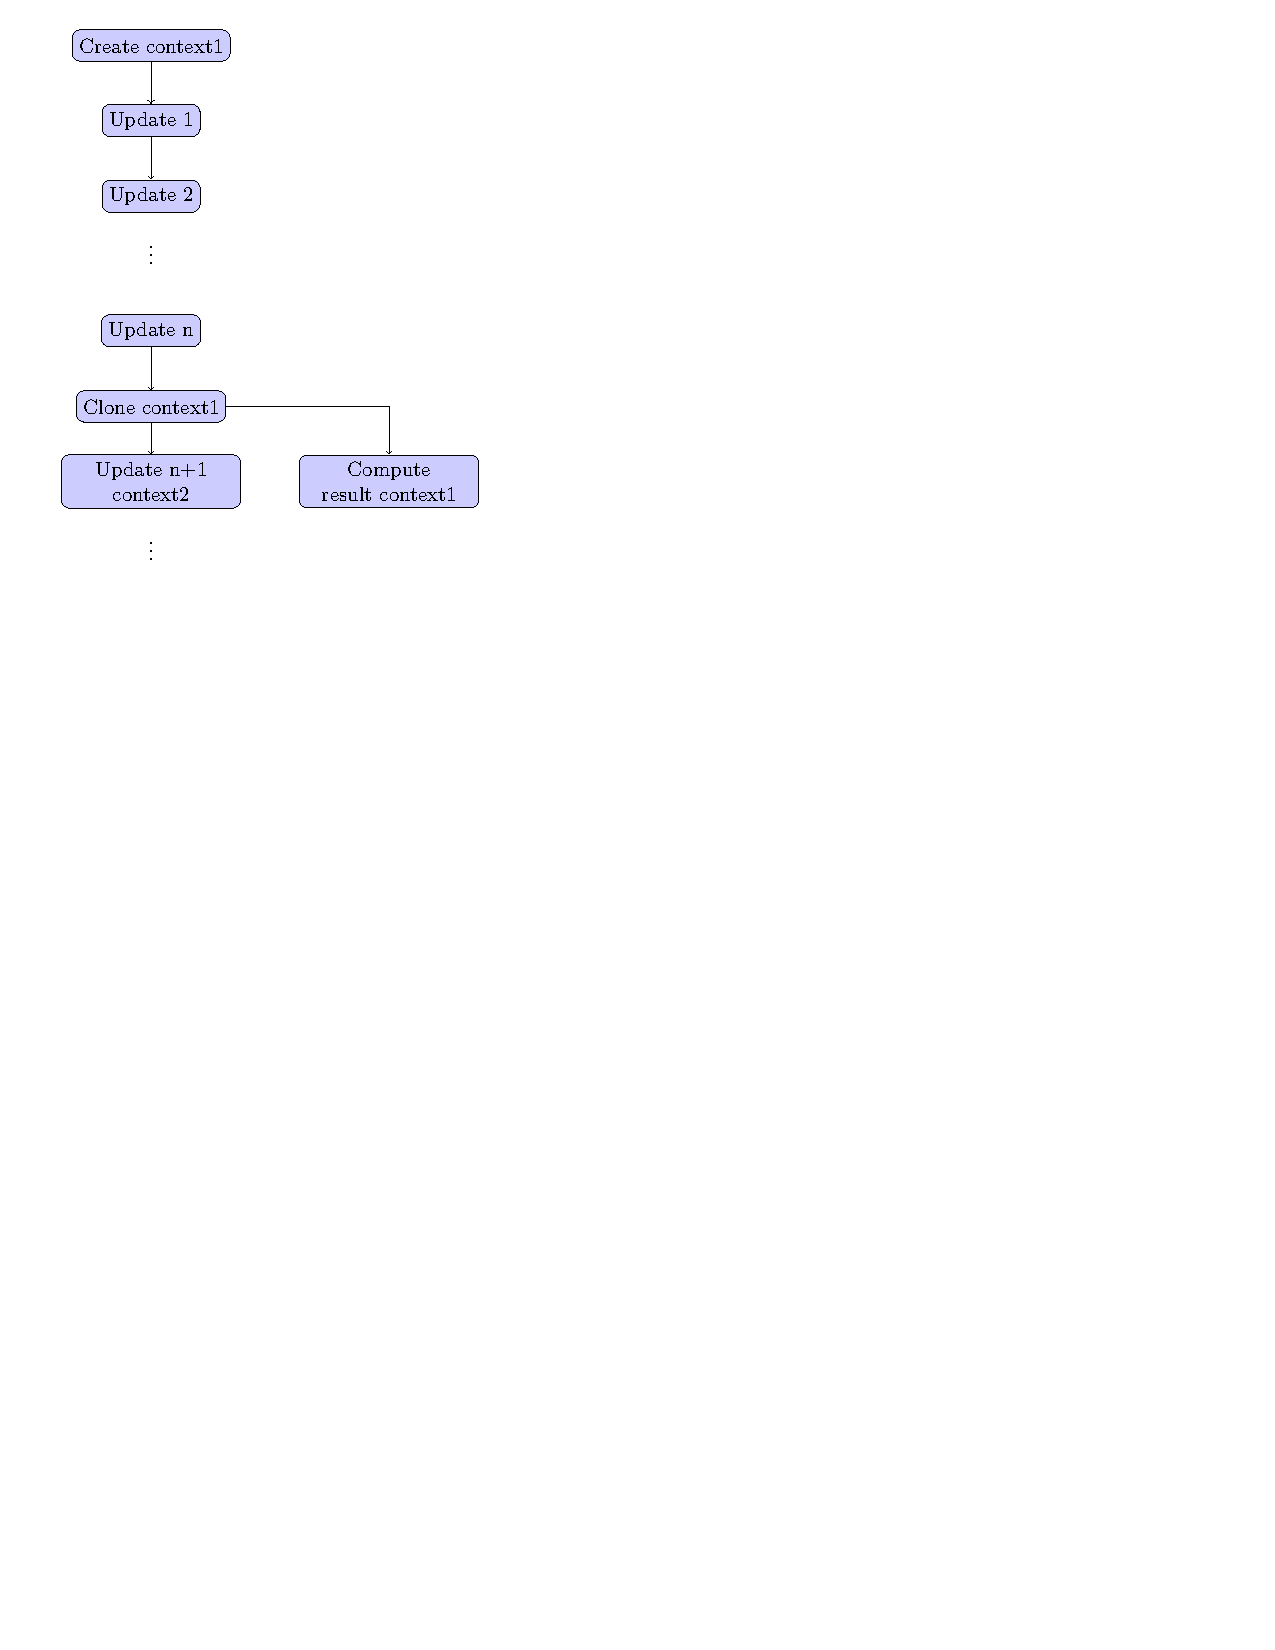
\includegraphics[trim=0cm 18.5cm 9.5cm 0cm,
height=10cm]{figures/hash_signature_clone.pdf}
\caption{Context - clone example\newline}
\label{fig:gci_clone}
%}
\end{figure}
As shown figure \ref{fig:gci_clone}, when we need to compute a result, but the
whole data added previously are needed for a future result, the solution is to clone the context, meaning that the whole
data added and the configuration is copied in another context.\newline
Then one context could be used to compute the result and the other one
to add other data when needed.\newline
\todo[inline]{What is it - why it's use - how to use - advantage - disadvantage}
\newpage
\section{Key management}
\label{gci_key_mng}
\todo[inline]{Add a short introduction of key management}
\todo[inline]{What is it - why it's use - how to use - advantage - disadvantage}
\subsection*{Generate a key}
\begin{figure}[!ht]
\centering
%\frame{
% trim: left, bottom, right, up
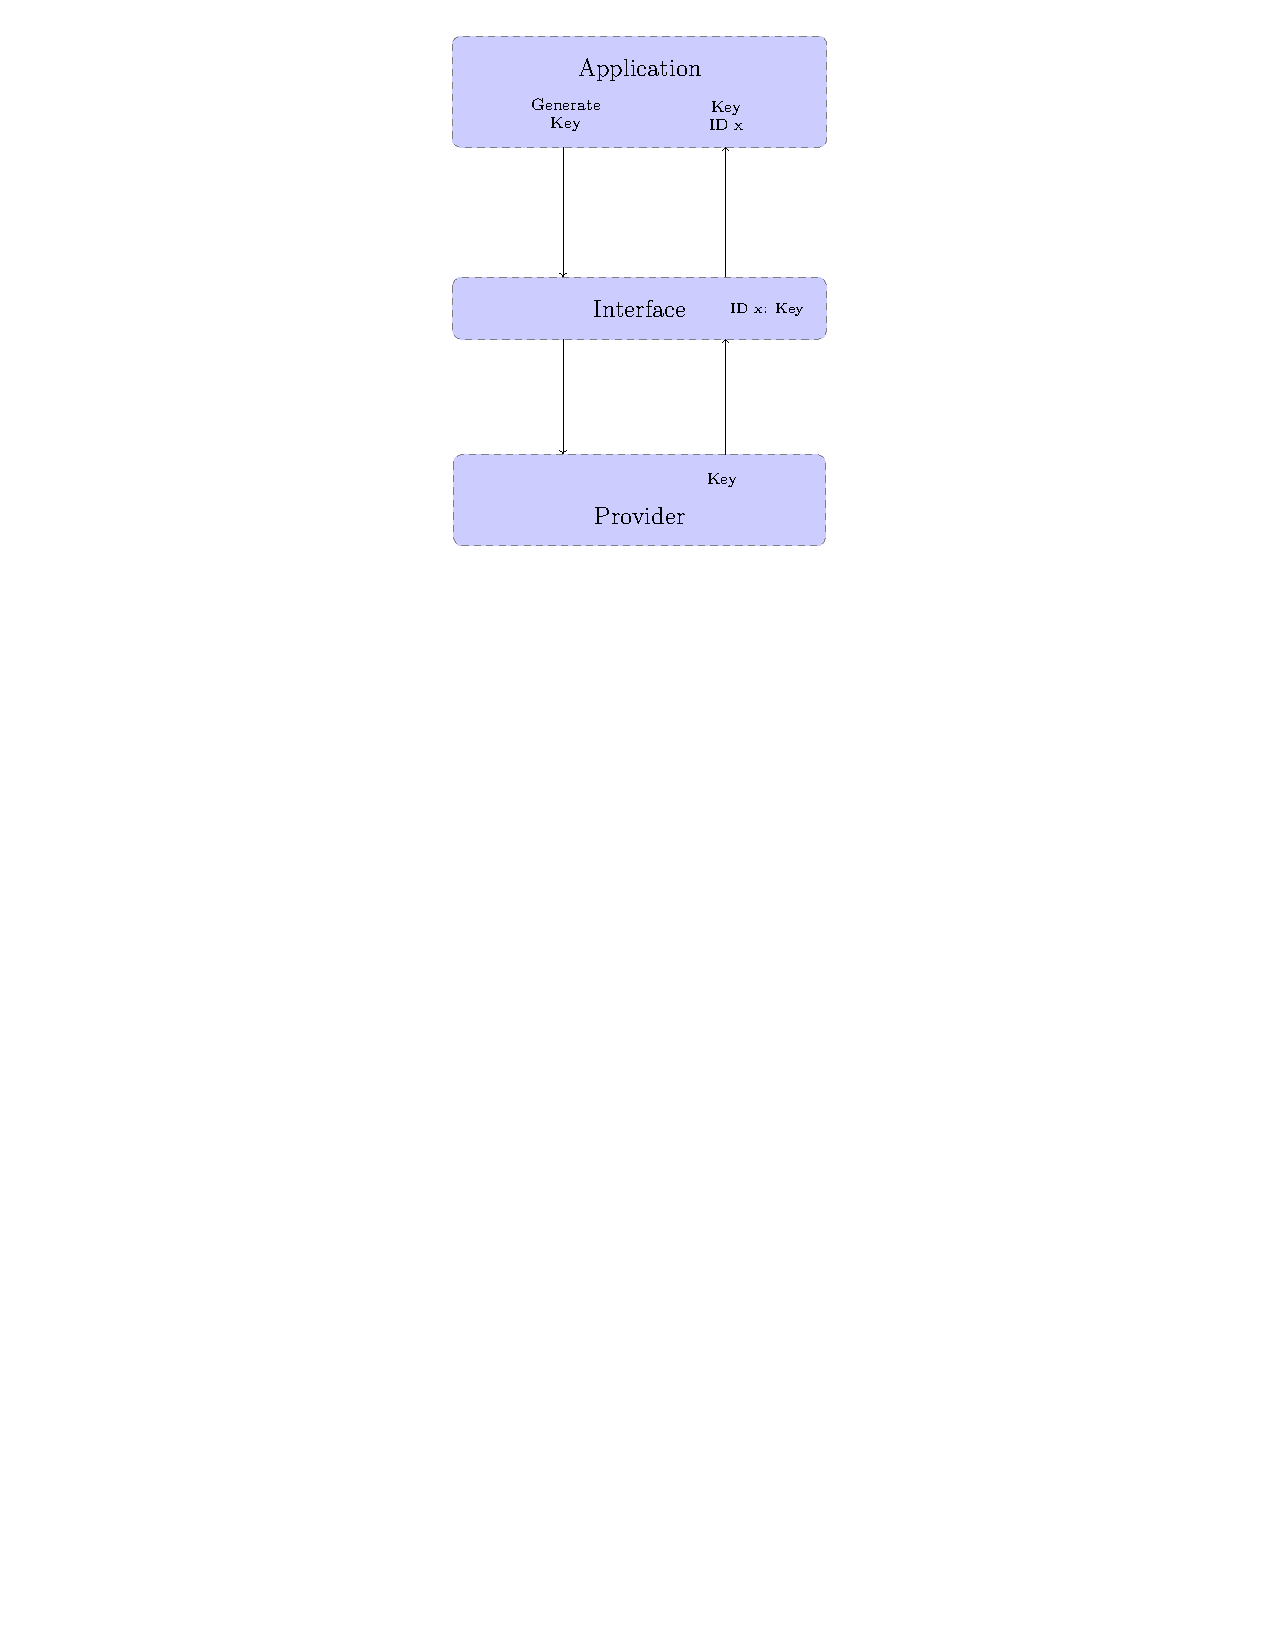
\includegraphics[trim=12cm 18.5cm 9.5cm 0cm,
height=10cm]{figures/key_manag_gen_key.pdf}
\caption{Key management - generate a key\newline}
\label{fig:gci_key_mng_gen}
%}
\end{figure}
\todo[inline]{Explain figure \ref{fig:gci_key_mng_gen}}
\newpage
\subsection*{Get a key}
\begin{figure}[!ht]
\centering
%\frame{
% trim: left, bottom, right, up
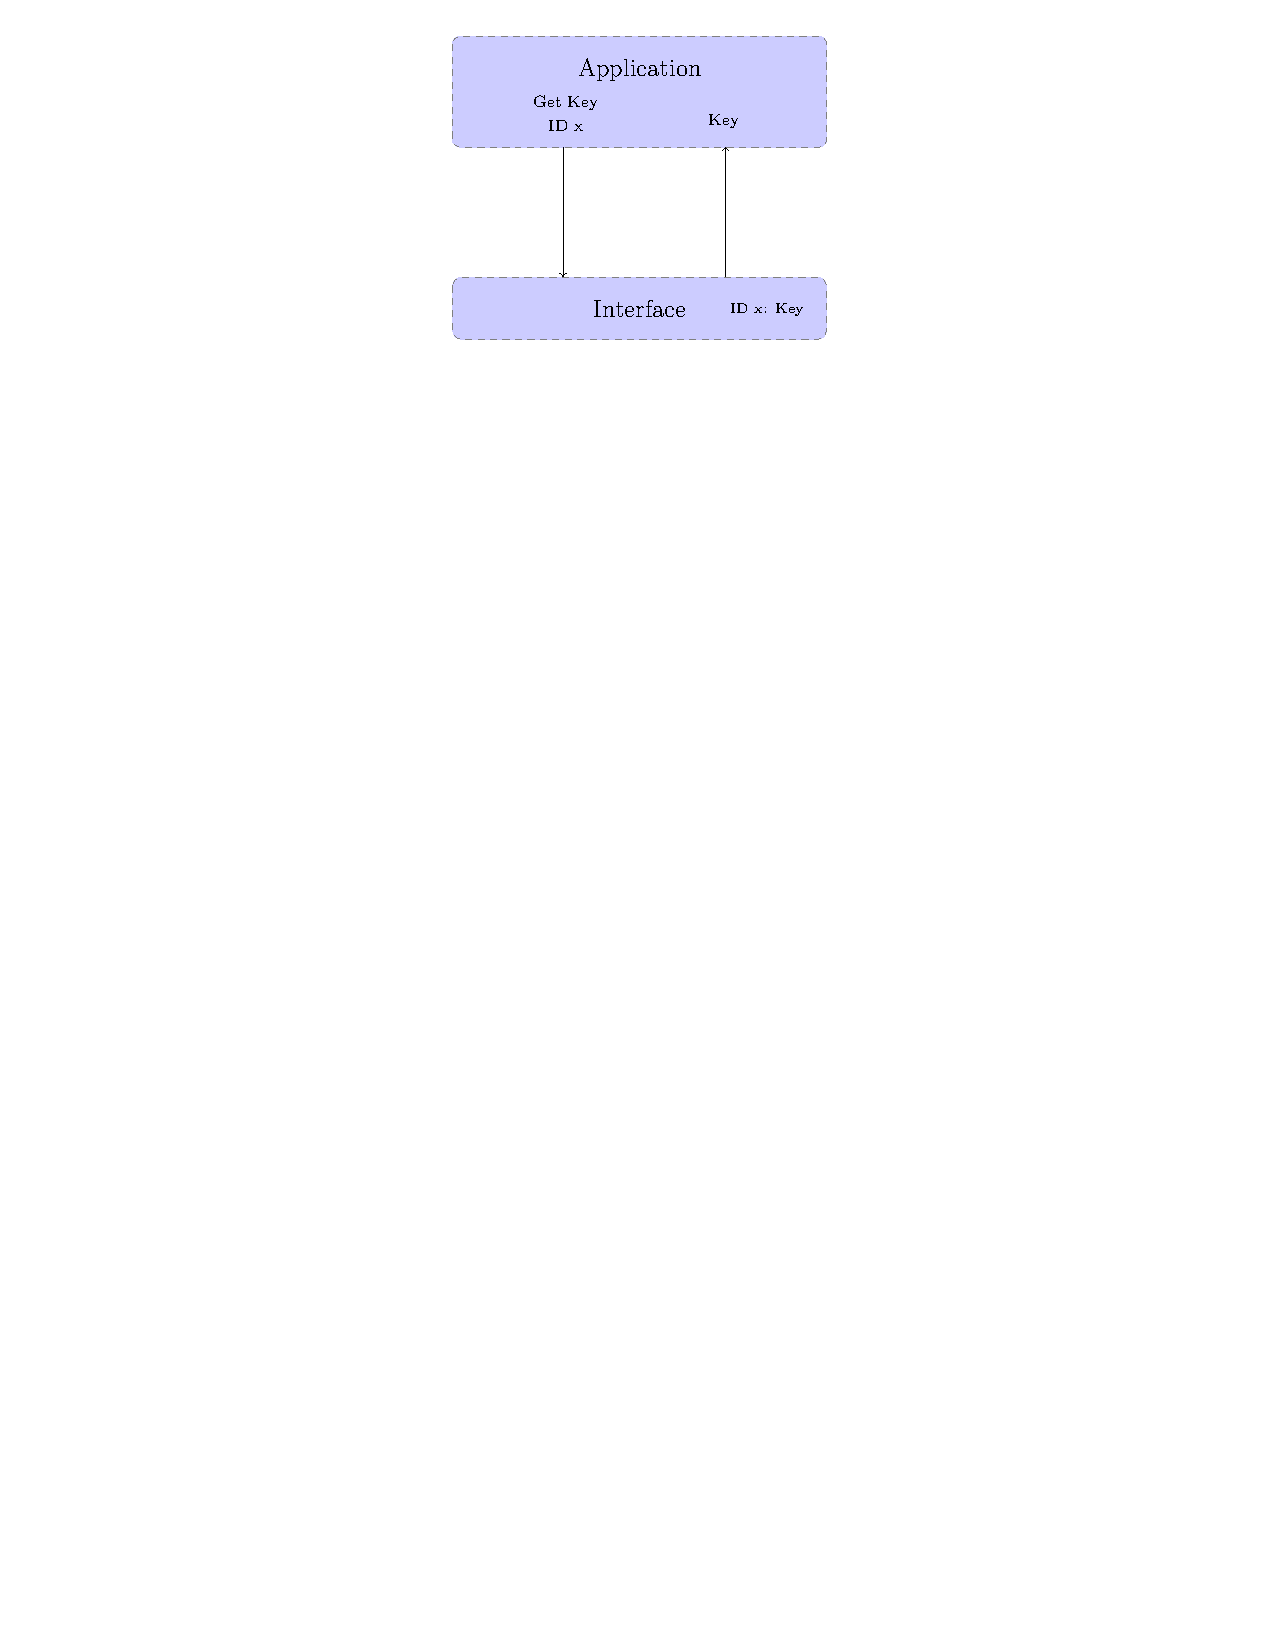
\includegraphics[trim=12cm 22cm 9.5cm 0cm]{figures/key_manag_get_key.pdf}
\caption{Key management - get a key\newline}
\label{fig:gci_key_mng_get}
%}
\end{figure}
\todo[inline]{Explain figure \ref{fig:gci_key_mng_get}}
\newpage
\subsection*{Delete a key}
\begin{figure}[!ht]
\centering
%\frame{
% trim: left, bottom, right, up
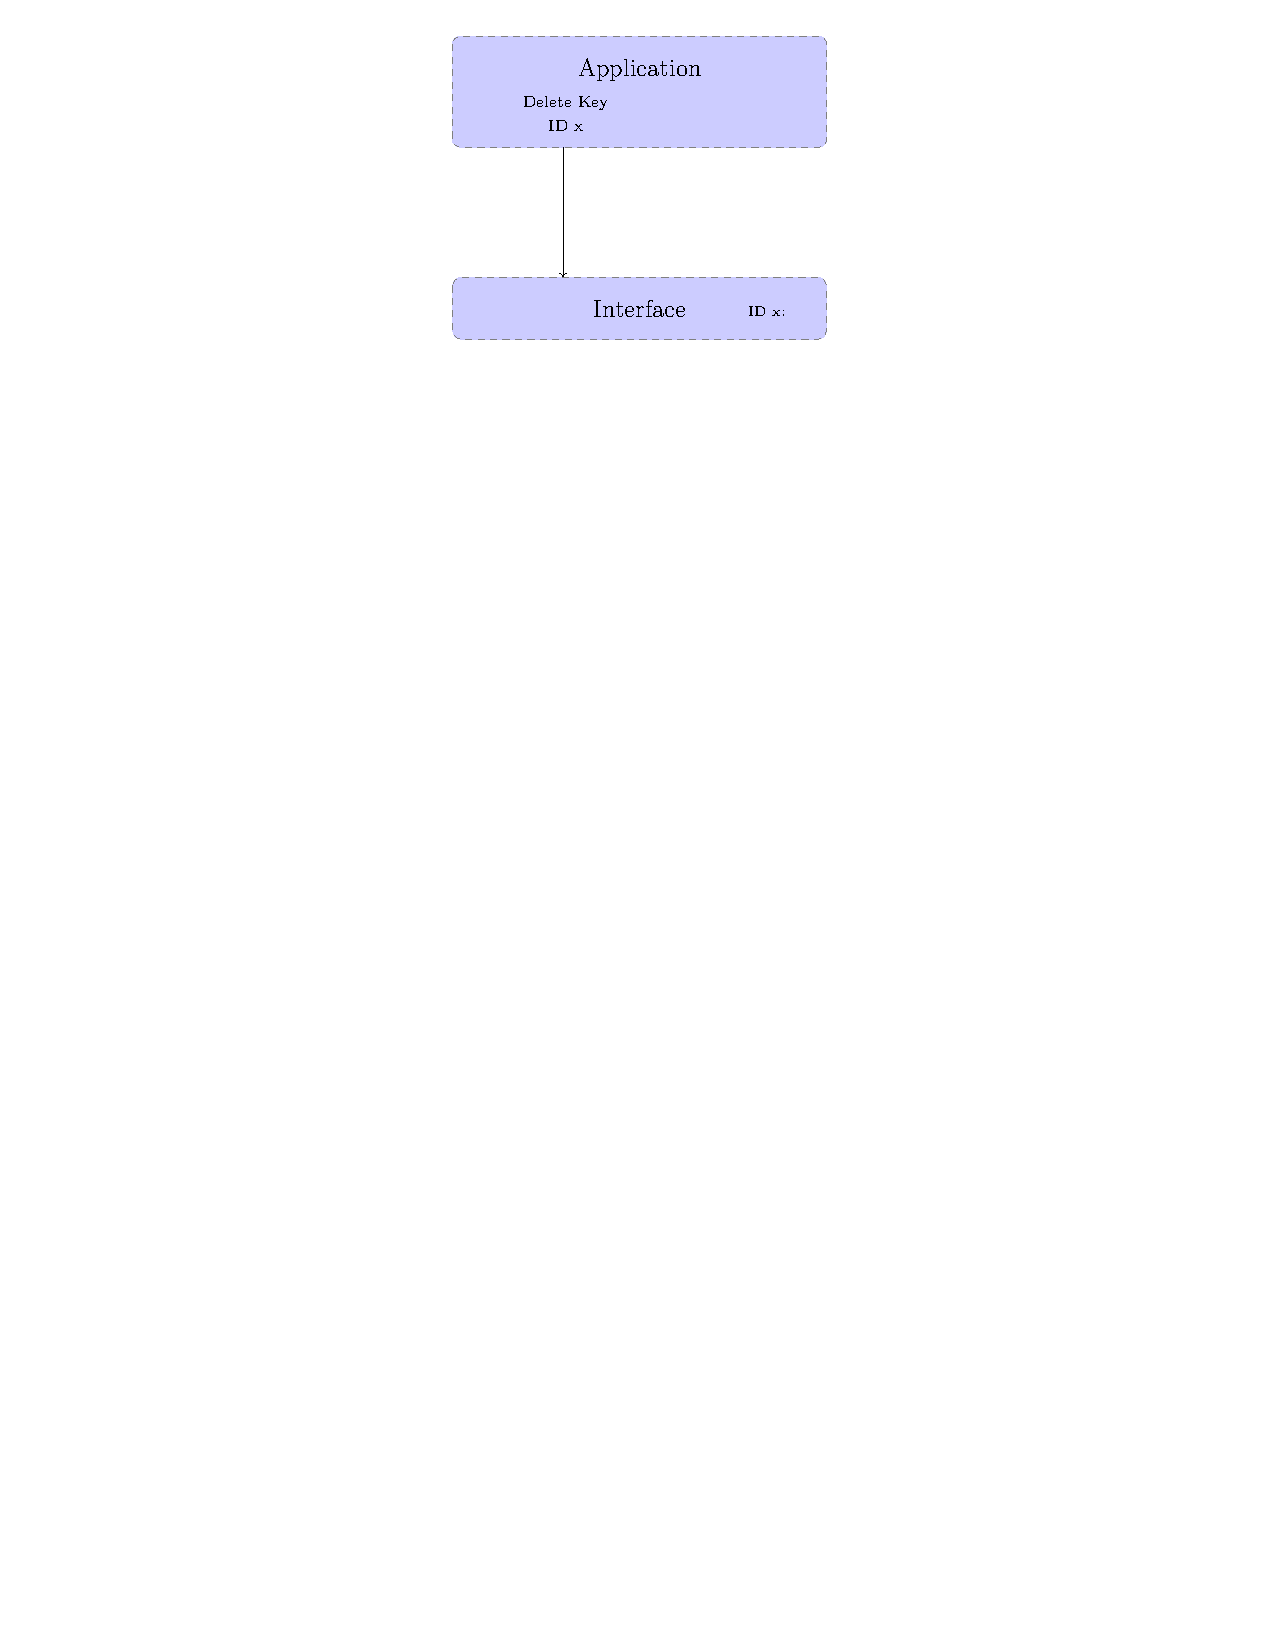
\includegraphics[trim=12cm 22cm 9.5cm 0cm]{figures/key_manag_del_key.pdf}
\caption{Key management - delete a key\newline}
\label{fig:gci_key_mng_del}
%}
\end{figure}
\todo[inline]{Explain figure \ref{fig:gci_key_mng_del}}
\newpage
\subsection*{Put a key}
\begin{figure}[!ht]
\centering
%\frame{
% trim: left, bottom, right, up
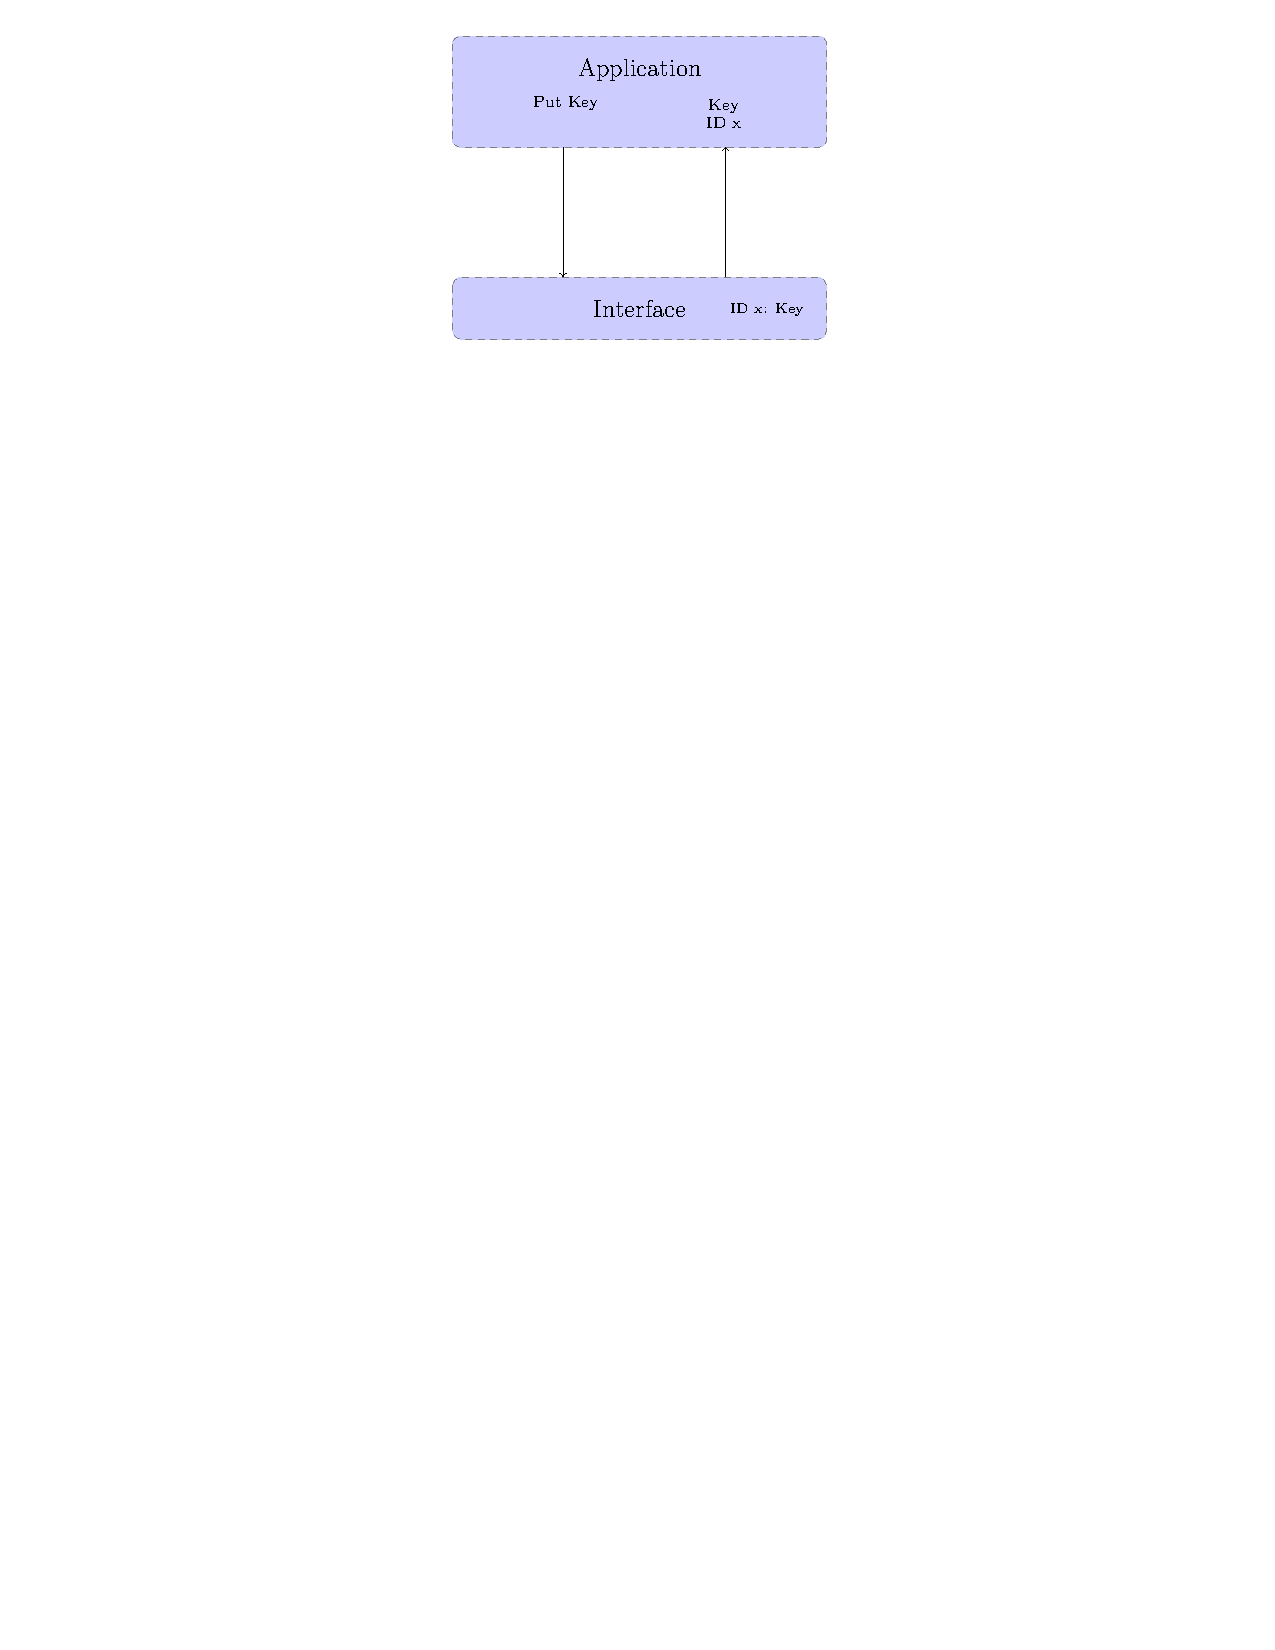
\includegraphics[trim=12cm 22cm 9.5cm 0cm]{figures/key_manag_put_key.pdf}
\caption{Key management - put a key\newline}
\label{fig:gci_key_mng_put}
%}
\end{figure}
\todo[inline]{Explain figure \ref{fig:gci_key_mng_put}}